\section{Einführung}
\subsection{Schaltungen}
Mittels der \textbf{Grosssignal}-Analyse wird das Bautal linearisiert und eine Gerade am Ursprung zB $R = \frac{U}{I}$ gelegt.
\begin{enumerate}[nosep]
	\item AC-Spannungsquellen durch Kurzschluss ersetzen
	\item AC-Stromquellen entfernen (Durch Leerläufe ersetzten)
	\item Kondensatoren entfernen (Unterbruch)
	\item Spulen Kurzsschliessen
	\item Nichtlineare Bauteile durch Kleinsignalersatzschaltung ersetzen
\end{enumerate}


Die \textbf{Kleinsignale}-Analyse leget eine Tangente am Arbeitspunkt an, anstatt einer Gerade am Ursprung. Schaltungen mit Kleinsignalen:
\begin{enumerate}[nosep]
	\item DC-Spannungsquellen durch Kurzschluss ersetzen
	\item DC-Stromquellen entfernen (Durch Leerläufe ersetzten)
	\item Kondensatoren Kurzschliessen
	\item Spulen entfernen (Unterbruch)
	\item Nichtlineare Bauteile durch Kleinsignale-Ersatzschaltungen ersetzten
\end{enumerate}

\subsection{Verstärkung}
Für Lineare Netzwerke können Eingangsspannungen mittels Superposition Überlagert und entsprechende Ausgangsspannungen berechnet werden.\\
\includegraphics[width=\linewidth]{Images/verstärker}

~\\
$k = \frac{\Delta V_{out}}{\Delta V_{in}}$\\
Für Nicht-Inventierender-Verstärker: $k = \frac{R_1 + R_F}{R_1}$ \\
Für Inventierender-Verstärker: $k = -\frac{R_F}{R_1}$

\subsection{Halbleiter}
Leitfähigkeit $\kappa$, Elementarladung $q = 1.6\cdot10^{-19}$ As zur Ladungsdichte $n$ und Beweglichkeit der Ladungsträger $\mu$.
\[
\kappa = \frac{1}{\varrho} = nq\mu
\]
Widerstand $R$ eines Materialsstücks mit Länge $l$, Querschnitt $A$ und der Materialkonstante $\varrho$:
\[
R = \rho \cdot \frac{l}{A} = \frac{l}{\kappa \cdot A}
\]
Temperaturabhängigkeit
\[
\varrho(T) = \varrho(T_0) \cdot (1 + \alpha(T - T_0))
\]

\includegraphics[width=\columnwidth]{Images/leitfähigkeit}

\subsection{Spannungsteiler}
\begin{minipage}{0.20\textwidth}
	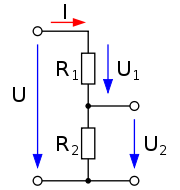
\includegraphics[width=\linewidth,keepaspectratio=true]{./Images/spannungsteiler}
\end{minipage}%%% to prevent a space
\begin{minipage}{0.30\textwidth}
	\begin{align*}
		\frac{U_2}{U} = \frac{R_2}{R_1 + R_2}
	\end{align*}
\end{minipage}

\subsection{Stromteiler}
\begin{minipage}{0.20\textwidth}
	
	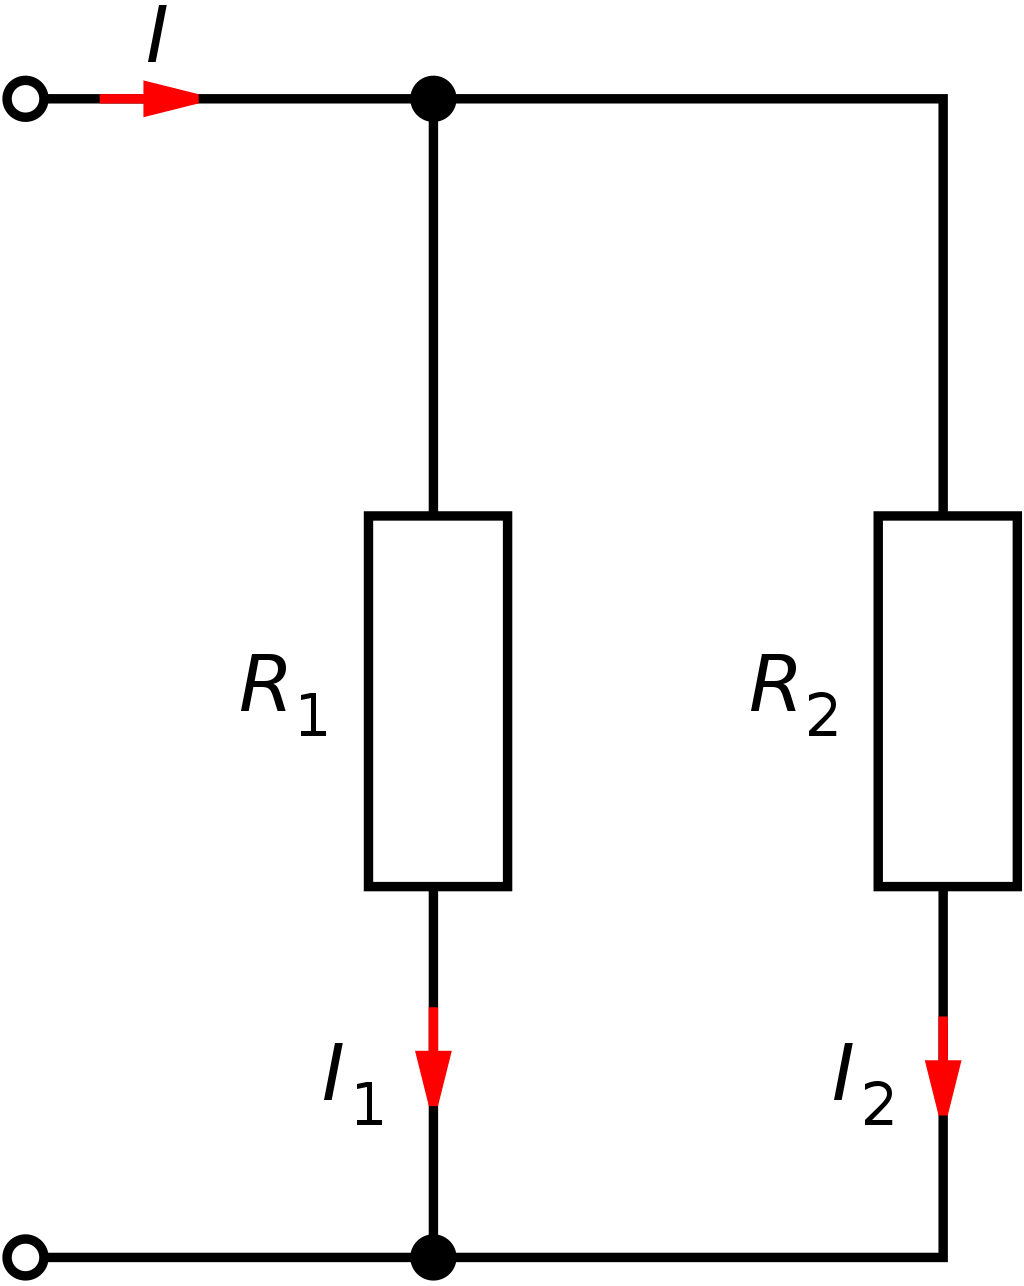
\includegraphics[width=0.8\linewidth,keepaspectratio=true]{./Images/stromteiler}
\end{minipage}%%% to prevent a space
\begin{minipage}{0.30\textwidth}
	\begin{align*}
		\frac{I_1}{I} = \frac{R_1//R_2}{R_1}
	\end{align*}
\end{minipage}

